\subsection{Generalized Logits}\label{sec:genlogit}

The generalized logit approach models the probabilities of the $m$ response categories directly as a set of \(m - 1\) logits.  These compare
each of the first \(m - 1\) categories to the last category, which serves
as the baseline.
The logits for any other pair of categories can be retrieved
from the \(m - 1\) fitted ones.

When there are $k$ predictors, \(x_1, x_2, \dots , x_k\),
which may be quantitative or categorical, the generalized logit
model expresses the logits as
\begin{eqnarray}\label{eq:glogit1}
  L_{jm}  \equiv
    \log \frac{\pi_{ij}}{\pi_{im}} & = & \beta_{0j}  +
  \beta _{1j} \,  x_{i1}  +
  \beta _{2j} \,  x_{i2}  + \cdots +
  \beta _{kj} \,  x_{ik} \quad
   j=1, \dots , m-1 \nonumber \\
  & = & {\vec{\beta}_j} \trans \vec{x}_i
\end{eqnarray}
Thus, there is one set of fitted coefficients, $\vec{\beta}_j$ for each
response category except the last.
Each coefficient, $\beta_{hj}$, gives the effect,
for a unit change in the predictor $x_h$,
on the log odds
that an observation belongs to category $j$, as opposed to category $m$.

The probabilities themselves are given by
\begin{equation*}
\pi_{ij} =
 \frac{ \exp ( {\vec{\beta}_j} \trans \vec{x}_i ) }
      { \sum_{i=1}^m \exp ( {\vec{\beta}_j} \trans \vec{x}_i ) }
 \period
\end{equation*}
Parameters in the $m-1$ equations \eqref{eq:glogit1} can be used to determine the
parameters or the predicted log odds for any pair of response categories
by subtraction.
For instance, for an arbitrary pair of categories, $a$ and $b$,
and two predictors, $x_1$ and $x_2$,
\begin{eqnarray*}%\label{eq:glogitab}
  L_{ab} & = & \log \frac{\pi_{ia}/\pi_{im}}{\pi_{ib}/\pi_{im}} \\
         & = & \log \frac{\pi_{ia}}{\pi_{im}} - \log \frac{\pi_{ib}}{\pi_{im}} \\
            & = & (\beta_{0a}-\beta_{0n}) + (\beta_{1a}-\beta_{1b}) x_{1i}
            + (\beta_{2a}-\beta_{2b}) x_{2i} 
\end{eqnarray*}
For example, the coefficient for $x_{1i}$ in $ L_{ab}$
is just $(\beta_{1a}-\beta_{1b})$.
Similarly, the predicted logit for any pair of categories
can be calculated as
\begin{equation*}
 \hat{L}_{ab} = \hat{L}_{am} - \hat{L}_{bm}
 \period
\end{equation*}

The generalized logit model cannot be fit using \PROC{LOGISTIC},
but it can be fit using \PROC{CATMOD}.%
\footnote{When one or more of the predictor variables are continuous,
however, you may have difficulty due to zero cell
frequencies, because \PROC{CATMOD} treats the data
as a contingency table.  In this case, it may help to reorder
the response variable so that the response category with the highest
frequency is the last, baseline category.
Alternatively, the continuous variable(s) can be collapsed into
categories so that populations with zero frequencies do not occur.}
An \ODS\ provides all predicted probabilities, and
the fitted logits.

\ixd{women's labor-force participation}
\begin{Example}[wlfpart2]{Women's labor-force participation}
To illustrate, we fit the generalized logit model to the
women's labor force participation data using the statements
below.
Husband's income is treated as a quantitative variable
by declaring it on the \stmt{direct}{CATMOD}.
\PROC{CATMOD} does not provide an overall test of the
whole model, however this can be carried out with a contrast
statement to test $H_0: \vec{\beta} = 0$.
\begin{listing}
proc catmod data=wlfpart;
   direct husinc;
   model labor = husinc children / noprofile noiter;
   response logits / out=results;
   contrast 'Husinc,Children=0'
      husinc   1,
      children 1;
\end{listing}

The maximum likelihood ANOVA table (\outref{out:wlfpart3.1}) shows that there are
two parameters fit for each regressor.
With a continuous predictor, the \LR{} test
of goodness-of-fit, which compares the current model to
the saturated model, is unreliable, because the contingency
table is very sparse.
\begin{Output}[htb]
\caption{Women's labor-force data, generalized logit model tests}\label{out:wlfpart3.1}
\small
\begin{output}
            MAXIMUM-LIKELIHOOD ANALYSIS-OF-VARIANCE TABLE

         Source                   DF   Chi-Square      Prob
         --------------------------------------------------
         INTERCEPT                 2        15.91    0.0004
         HUSINC                    2        12.82    0.0016
         CHILDREN                  2        53.98    0.0000

         LIKELIHOOD RATIO         86       138.67    0.0003
\end{output}
\end{Output}

The table of parameter estimates, shown in \outref{out:wlfpart3.2}, contains the coefficients
for the two fitted logits,
\begin{eqnarray}
  \log \left( \frac{ \Pr ( \mbox{fulltime} ) }
  { \Pr ( \mbox{not working} ) } \right)  & = &
  0.7035 - 0.0972 \,  \mbox{H\$} + 1.2793 \,  \mbox{kids} \label{eq:wlfgen1}\\
%
  \log \left( \frac{ \Pr ( \mbox{parttime} ) }
  { \Pr ( \mbox{not working} ) } \right) & = &
  -1.4216 + 0.00689 \,  \mbox{H\$} - 0.0107 \,  \mbox{kids} \label{eq:wlfgen2}
\end{eqnarray}
The predicted log odds for working fulltime as opposed to parttime
are therefore given by
\begin{equation}\label{eq:wlfgen3}
  \log \left( \frac{ \Pr ( \mbox{fulltime} ) }
  { \Pr ( \mbox{not working} ) } \right)  =
  2.1251 - 0.1041 \,  \mbox{H\$} + 1.29 \,  \mbox{kids}
\end{equation}
The coefficients in \eqref{eq:wlfgen1}, \eqref{eq:wlfgen2} and \eqref{eq:wlfgen3}
are not directly comparable to those in
\eqref{eq:wlfnest1} and \eqref{eq:wlfnest2} for the nested
dichotomies models, because they pertain to different comparisons.
\begin{Output}[htb]
\caption{Women's labor-force data, generalized logit model parameter estimates}\label{out:wlfpart3.2}
\small
\begin{output}
              ANALYSIS OF MAXIMUM-LIKELIHOOD ESTIMATES

                                         Standard    Chi-
  Effect            Parameter  Estimate    Error    Square   Prob
  ----------------------------------------------------------------
  INTERCEPT                 1    0.7035    0.4140     2.89  0.0892
                            2   -1.4216    0.4528     9.86  0.0017
  HUSINC                    3   -0.0972    0.0281    11.98  0.0005
                            4   0.00689    0.0235     0.09  0.7689
  CHILDREN                  5    1.2793    0.1811    49.90  0.0000
                            6   -0.0107    0.2345     0.00  0.9635
\end{output}
\end{Output}

A plot of the predicted probabilities of the three categories of
\texttt{labor} is easily obtained from the \texttt{results}
\Dset\ produced by \PROC{CATMOD}.
This \Dset\ contains both fitted probabilities (\verb|_type_='PROB'|)
and fitted logits (\verb|_type_='FUNCTION'|), so we select the
\verb|_type_='PROB'| observations with a \texttt{where} statement.
\begin{listing}
proc gplot data=results;
   where (_type_='PROB');
   plot _pred_ * husinc = labor /
      vaxis=axis1 hm=1 vm=1 anno=labels nolegend;
   by children;
   axis1 order=(0 to .9 by .1) label=(a=90);
   symbol1 i=join v=circle   c=black;
   symbol2 i=join v=square   c=red;
   symbol3 i=join v=triangle c=blue;
   label _pred_='Fitted probability';
\end{listing}
The fitted probabilities are shown in \figref{fig:wlfpart3}.
When there are no young children in the home, a woman's probability
of not working rises sharply with husband's income, while her
probability of working full time declines sharply, and her
probability of working part time increases modestly.
With children present, the direction of these relations with husband's
income are the same, but the levels of not working and full
time work are reversed.
%% two subfigures side-by-side
\begin{figure}[htb]
 \begin{minipage}[b]{.49\linewidth}
  \centering
  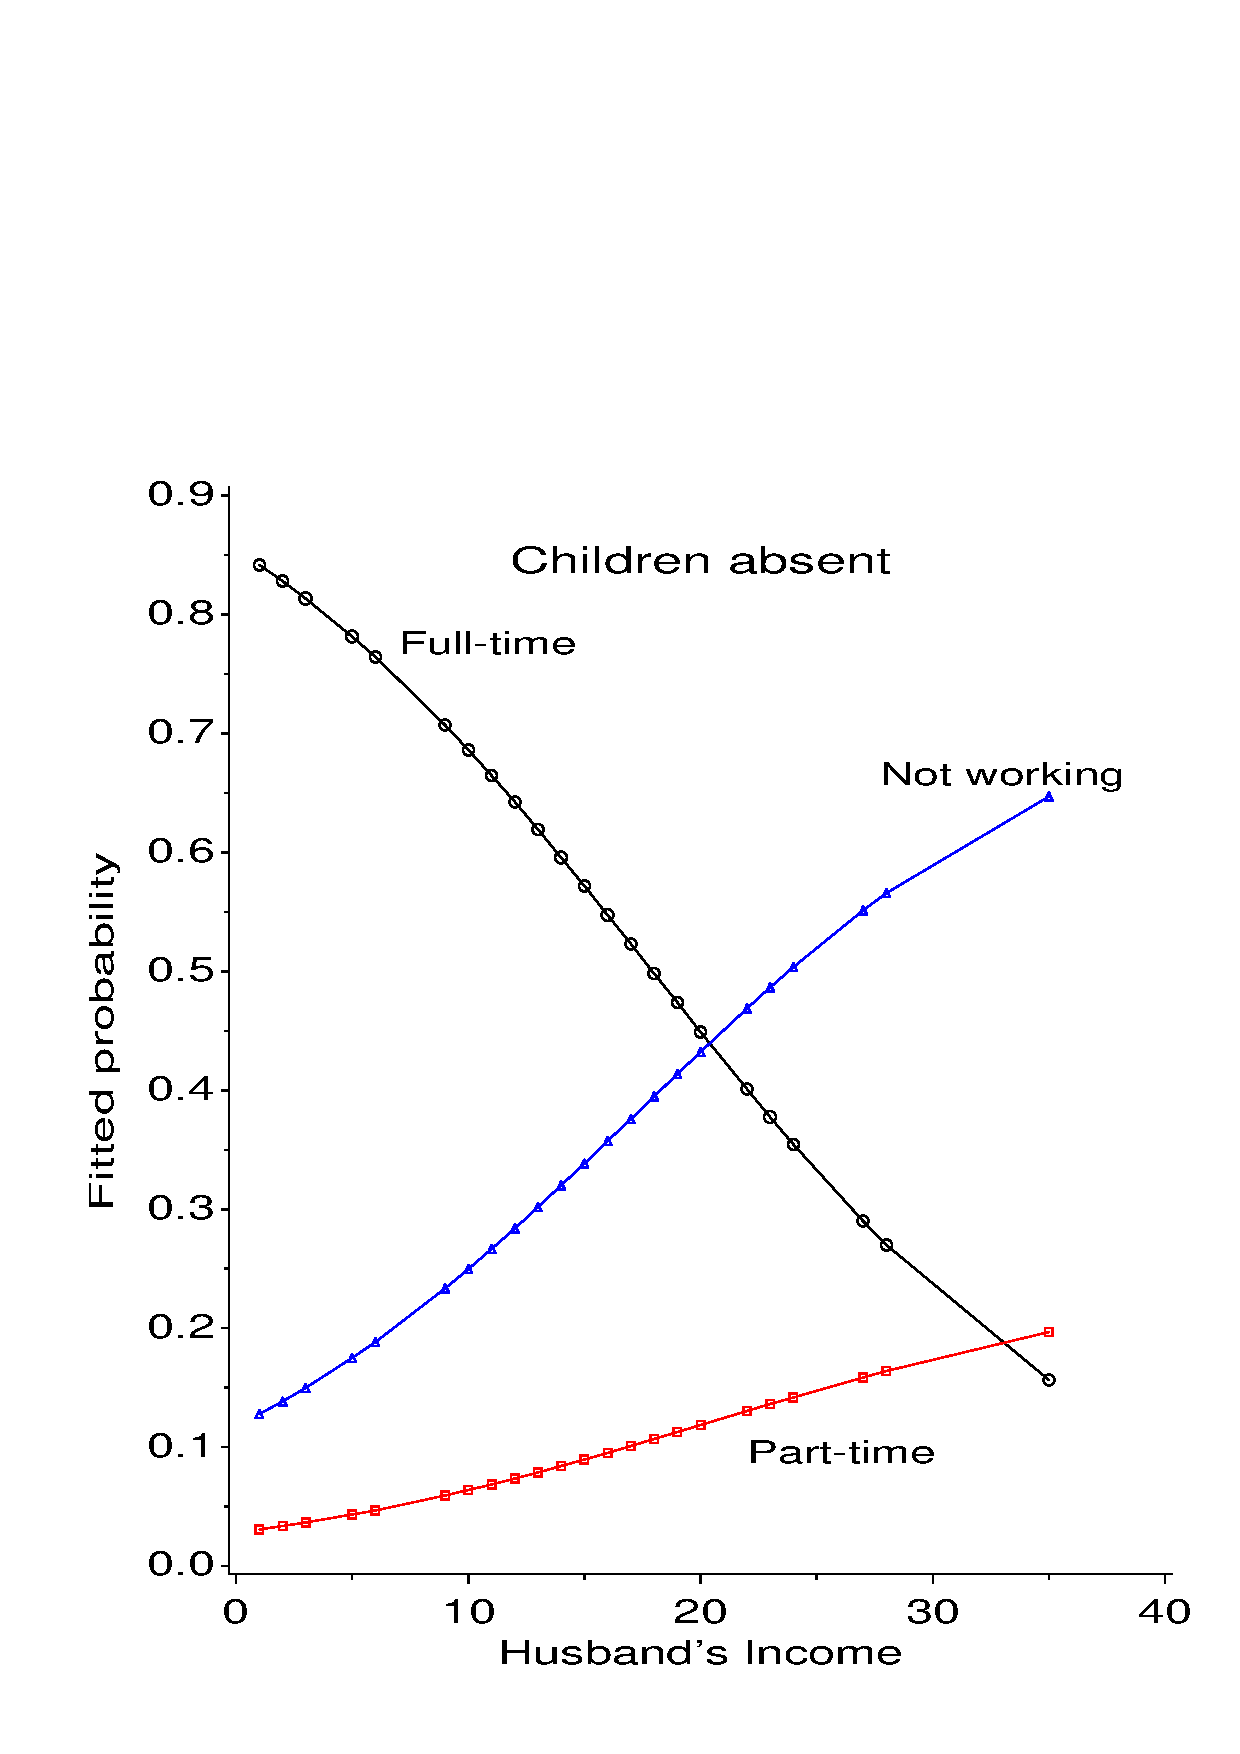
\includegraphics[width=1\linewidth]{ch6/fig/wlfpart31}
 \end{minipage}%
 \hfill
 \begin{minipage}[b]{.49\linewidth}
  \centering
  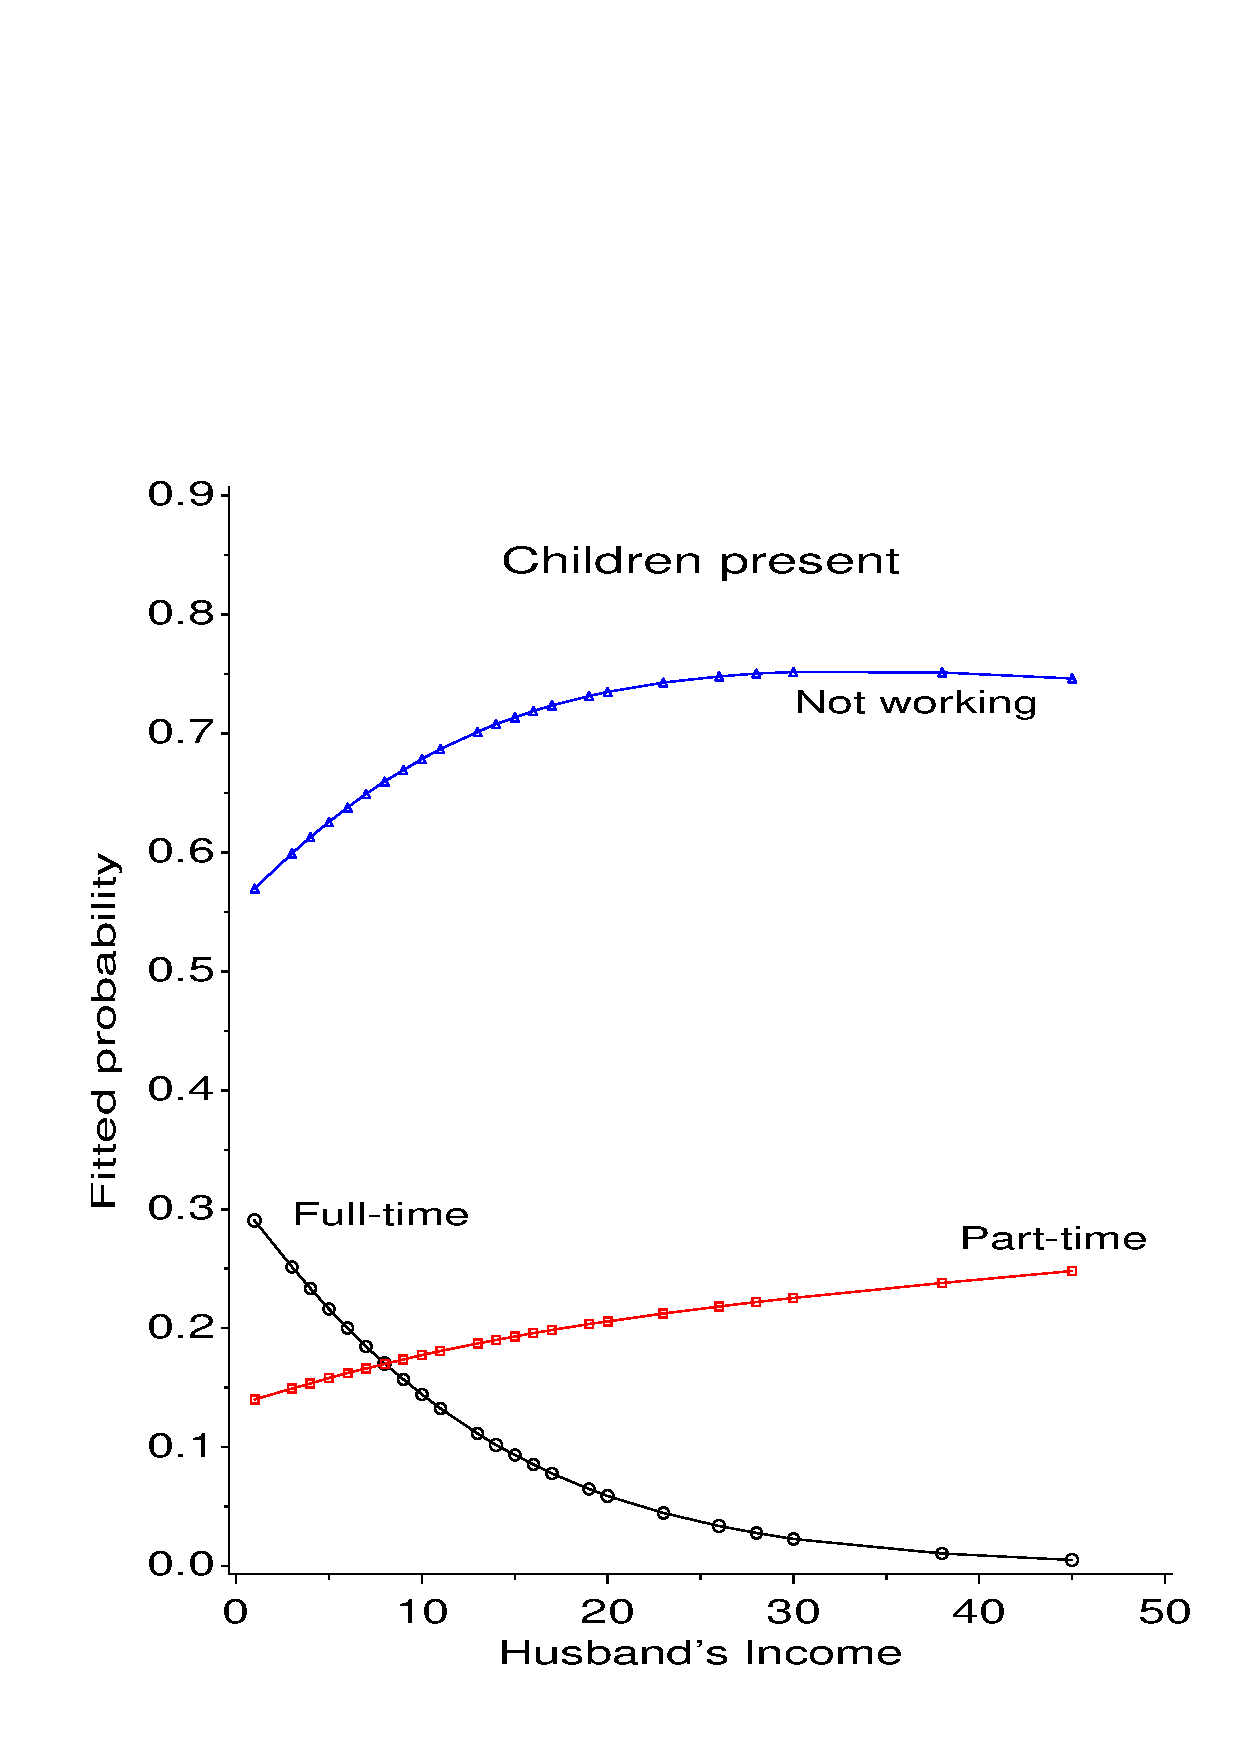
\includegraphics[width=1\linewidth]{ch6/fig/wlfpart32}
 \end{minipage}
  \caption[Women's Labor Force Participation, fitted probabilities]{Fitted probabilities for the generalized logit model}\label{fig:wlfpart3}
\end{figure}
Plots similar to \figref{fig:wlfpart3} can be produced with the
\macro{CATPLOT}.  These statements would plot predicted probabilities
(\pname{TYPE=PROB}) in the \pname{RESULTS} \Dset\ with separate
curves for each working category (\pname{CLASS=LABOR}),
and separate panels for those with and without children
(\pname{BYVAR=CHILDREN}).  These plots are not shown to conserve space.
\begin{listing}
axis1 order=(0 to .9 by .1) label=(a=90 'Fitted probability');
axis2 offset=(1,10pct);

%catplot(data=results, x=husinc, y=_pred_, type=PROB,
   class=labor, clfmt=labor.,
   byvar=children, byfmt=kids.);
\end{listing}
To plot the predicted log odds corresponding to \eqref{eq:wlfgen1}--\eqref{eq:wlfgen3} takes slightly more work, because the
\ODS\ from \PROC{CATMOD} contains only the first two predicted logits.
The following steps calculate the logit for \eqref{eq:wlfgen3} from the other
two and uses the \macro{CATPLOT} to plot the results, as shown in
\figref{fig:wlfpart35}.

%% two subfigures side-by-side
\begin{figure}[htb]
 \begin{minipage}[b]{.49\linewidth}
  \centering
  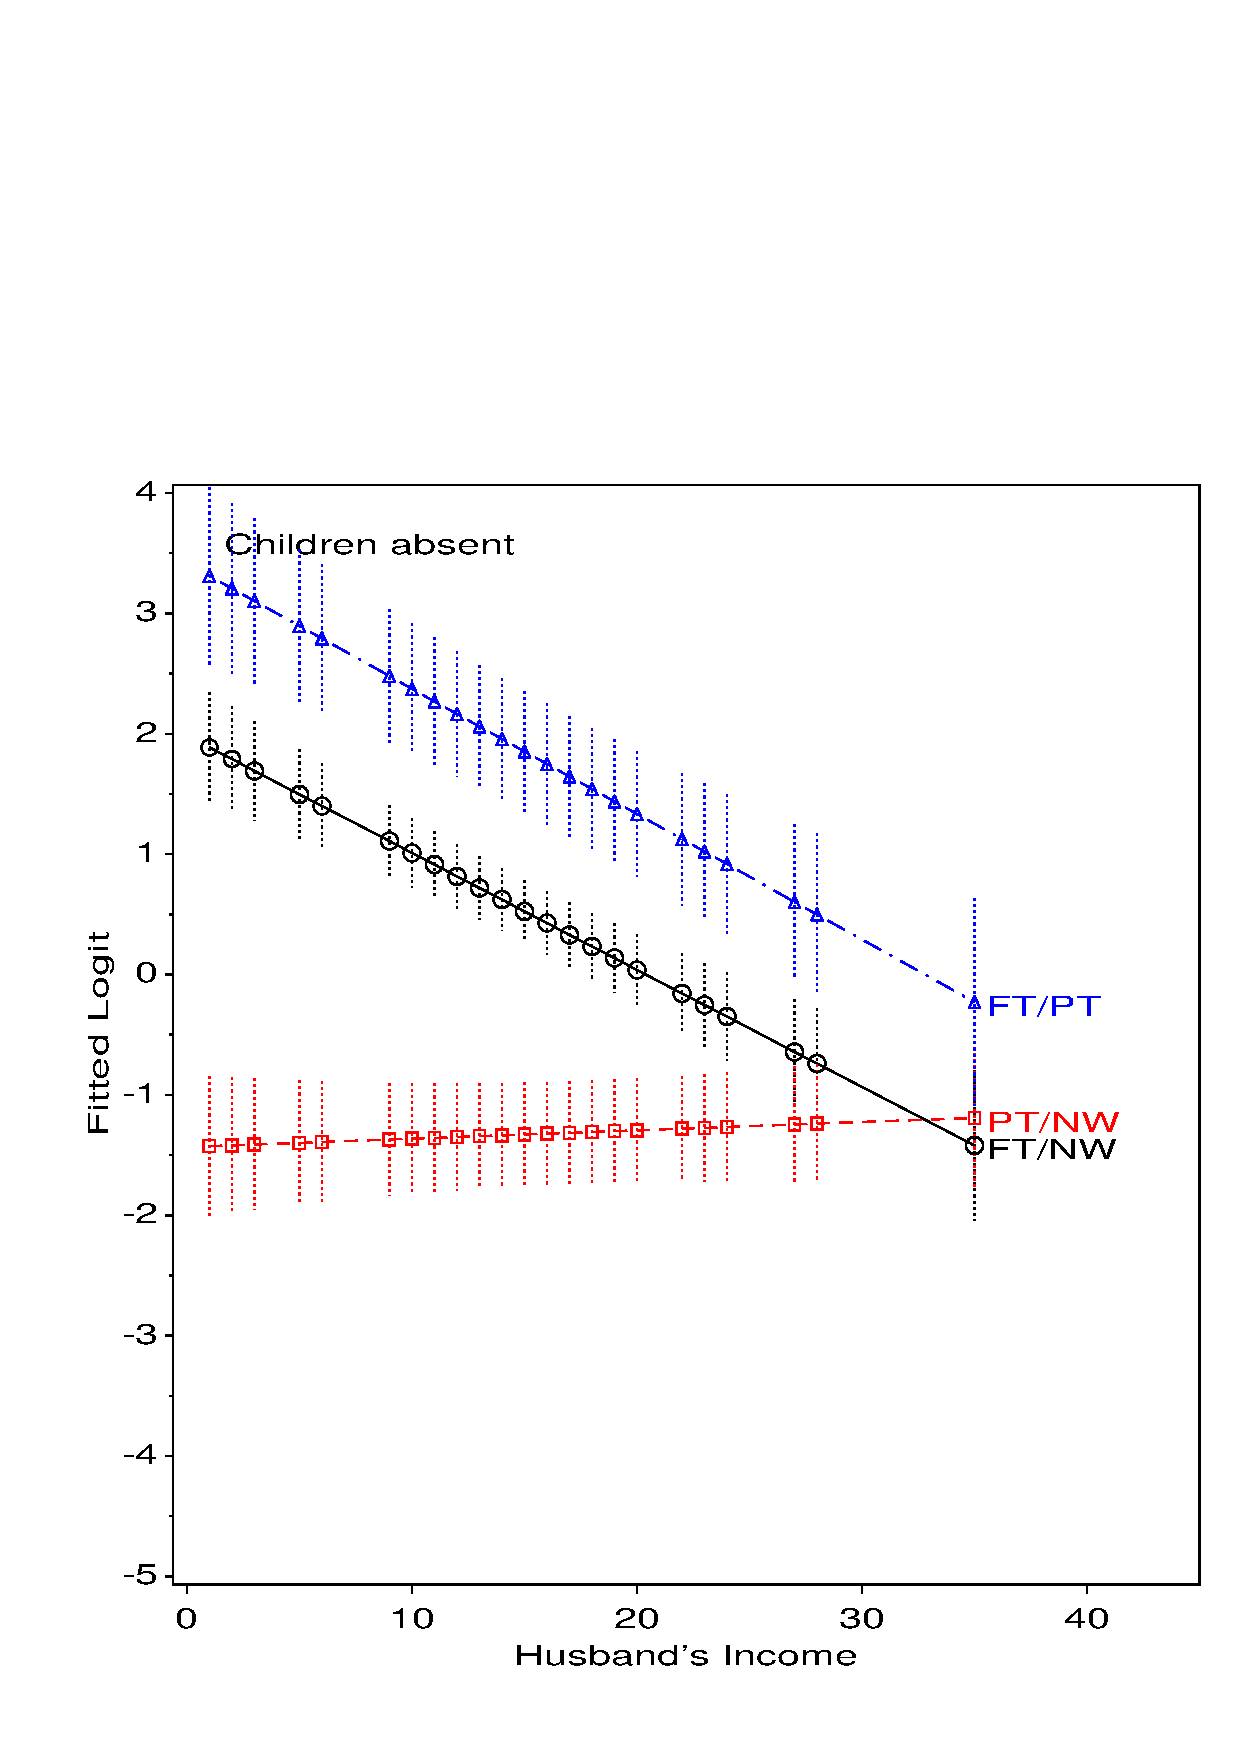
\includegraphics[width=1\linewidth]{ch6/fig/wlfpart35}
 \end{minipage}%
 \hfill
 \begin{minipage}[b]{.49\linewidth}
  \centering
  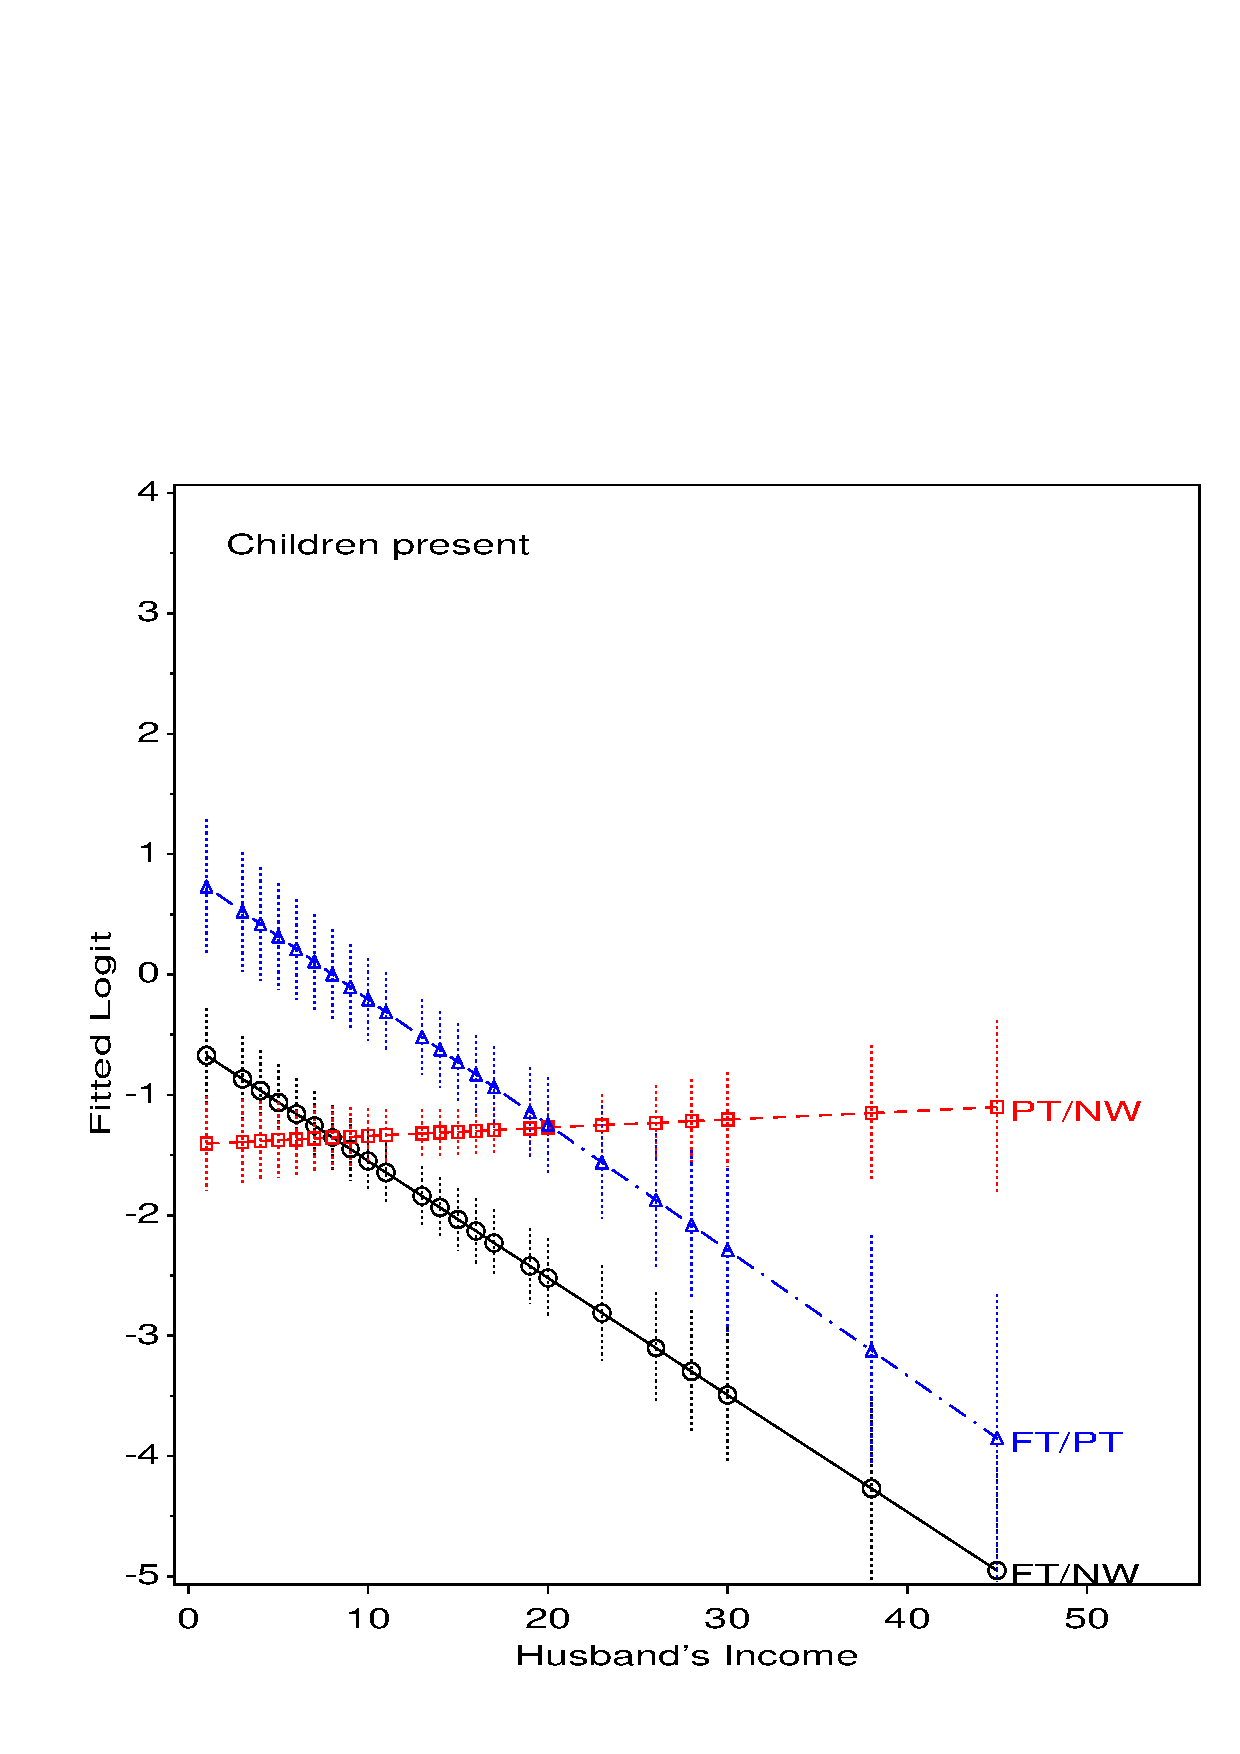
\includegraphics[width=1\linewidth]{ch6/fig/wlfpart36}
 \end{minipage}
  \caption[Women's Labor Force Participation, fitted log odds]{Fitted log odds for the generalized logit model}\label{fig:wlfpart35}
\end{figure}
\begin{listing}
proc format;
   value num 1='FT/NW'  2='PT/NW'  3='FT/PT';
data logits;
   set results(rename=(_number_=logit));
   by _sample_;
   format logit num.;
   where (_type_='FUNCTION');
   retain logit1 logit2 se1 se2;
   drop labor logit1 logit2 se1 se2;
   if first._sample_
      then do; logit1 = _pred_; se1=_sepred_; end;
      else do; logit2 = _pred_; se2=_sepred_; end;
   output;
   logit=3;
   _pred_ = logit1 - logit2;
   _sepred_ = sqrt(se1**2 + se2**2);
   if last._sample_ then output;

axis1 label=(a=90 'Fitted Logit') order=(-5 to 4);
%catplot(data=logits, x=husinc, y=_pred_, class=logit,
   byvar=children, byfmt=kids.);
\end{listing}
\end{Example}
